\documentclass[a4paper,10pt]{article}
\usepackage[utf8]{inputenc}

\setlength\parindent{0pt}
\usepackage[english]{babel}
\usepackage[dvinames]{xcolor}
\usepackage[compact,small]{titlesec}
\usepackage{booktabs}
\usepackage{multirow}
\usepackage{amsfonts,amsmath,amssymb}
\usepackage{marginnote}
\usepackage[top=1.8cm, bottom=1.8cm, outer=1.8cm, inner=1.8cm, heightrounded, marginparwidth=2.5cm, marginparsep=0.5cm]{geometry}
\usepackage{enumitem}
\setlist{noitemsep,parsep=2pt}
\newcommand{\highlight}[1]{\textcolor{kuleuven}{#1}}
\usepackage{pythonhighlight}
\usepackage{cleveref}
\usepackage{graphicx}
\usepackage{algorithmic}
\usepackage{tabularx}

\newcommand{\nextyear}{\advance\year by 1 \the\year\advance\year by -1}
\newcommand{\thisyear}{\the\year}
\newcommand{\deadlineGroup}{November 27, \thisyear{} at 16:00 CET}
\newcommand{\deadlineCode}{December 18, \thisyear{} at 16:00 CET}
\newcommand{\deadlineReport}{January 4, \nextyear{} at 16:00 CET}

\newcommand{\ReplaceMe}[1]{{\color{blue}#1}}
\newcommand{\RemoveMe}[1]{{\color{purple}#1}}

\setlength{\parskip}{5pt}

%opening
\title{Artificial Neural Networks: Exercise session 1}
\author{Stijn Staring (r0620003)}

\begin{document}
\fontfamily{ppl}
\selectfont{}

\maketitle

%\section{\RemoveMe{Formal requirements}} \label{sec_this}

\section{Exercises of Section 2}
\textbf{Function approximation: comparison of various algorithms:
	Take the function $y = sin(x2) for x = 0 : 0:05 : 3$ and try to approximate it using a neural network with one hidden
	layer. Use different algorithms. How does gradient descent perform compared to other training algorithms?}\\

\textbf{Learing from target data without noise}\\
The neural network that is used in this section consists of one hidden layer with $ 50 $ hidden neurons and a single input and output neuron. The input data is a 1D array of $ 189  $values. \\

%\textbf{Gradient descent vs Gradient descent with adaptive learning rate}\\
The gradient descent and the gradient descent with adaptive learning rate behave very similar for the first $ 15 $ iterations. Where they give both unsatisfactory results with a correlation coefficient between predictions and targets of only $ R = 0.08 $. Quality of the regression improves when $ 1000 $ epochs are performed. Here clearly the method of gradient descent with adaptive learning rate to update the weights performs better. The correlation coefficient of gradient descent with and without adaptive learning rate are respectively $ R = 0.535 $ and $ R = 0.857 $. All the results of the different methods to learn from noiseless data that further are discussed, are summarized by Table \ref{tab:corr_no_noise}. The calculation of the MSE is made by considering $ 3142 $ samples of the sinus function without noise. \\

It can be seen that all other methods behave equally bad as gradient descent when only $ 1 $ epoch is performed except for the Levenberg-Marquardt method and bayesian regularization backpropagation method. Already after one epoch is achieves a higher correlation between prediction and target values than both the gradient methods after $ 1000 $ epochs. After $ 15 $ epochs they achieve as only methods perfect linear correlation.\\ 

It should be noted that the disadvantage of the gradient descent method in comparison with other methods is that it has slow convergence in function of the amount of iterations in comparison with methods that are derivatives from the Newton method as for example the BFGS quasi Newton algorithm and Levenberg-Marquardt algorithm. One iteration of the later mentioned algorithms takes longer than one iteration of the Gradient descent. Using the amount of epochs as stopping criteria works therefore in the advantage of update methods that converge fast in function of the amount of iterations. Therefore, it is expected that when a time limit is used as stopping criteria this will be in favour of the gradient descent method, because one iteration is less calculation expensive. \\

\begin{table}
	\centering
	\begin{tabular}{@{}l|lccr@{}} \toprule
		\textbf{Learning rule}    & $ 1 $ epoch & $ 15 $ epochs & $ 1000 $ epochs & MSE \\\midrule
		\textbf{Gradient Descent}    & $ 0.0773 $  & $ -0.0818 $  & $ 0.575 $ & $ 3.30\times10^{-1} $ \\
		\textbf{GD with adaptive learning rate} & $ 0.0773 $  & $ -0.0697 $  & $ 0.863 $ & $ 1.20\times10^{-1} $  \\
		\textbf{Fletcher-Reeves} & $ 0.00198 $  & $ 0.790 $  & $ 0.999 $ & $ 1\times10^{-3} $ \\
		\textbf{Polak-Ribier} & $ -0.0464 $  & $ 0.758 $  & $ 0.999 $ & $ 1\times10^{-3} $  \\
		\textbf{BFGS} & $ -0.0625 $  & $ 0.857 $  & $ 1.00 $ & $ 0.0 $ \\
		\textbf{Levenberg-Marquardt} & $ 0.899 $  & $ 1.00 $  & $ 1.00 $ & $ 0.0 $ \\
		\textbf{Bayesian Regularization Backpropagation} & $ 0.837 $  & $ 1.00 $  & $ 1.00 $ & $ 0.0 $ \\ \bottomrule
	\end{tabular}
	\caption{Correlation coefficients and MSE between predictions and targets of  different methods in function of the amount of epochs performed during training on noiseless data.}
	\label{tab:corr_no_noise}
\end{table}

%The performance of further methods with respect to the correlation coefficient is given in table \ref{tab:corr_no_noise} Using the ``Fletcher-Reeves'' conjugate gradient algorithm to update the weights decisevely outperforms a simple gradient descent in function of the amount of epochs. Already after $ 15 $ epochs a correlation coefficient of $ R = 0.736 $ is achieved and after $ 1000 $ epochs there is almost perfect regression with $ R = 0.99 $.\\

\textbf{Learing from target data without noise}\\
Now instead of performing a regression with a feedforward neural network on noiseless target data now additional noise is added by adding gaussian noise with a standard deviation of $ 0.2 $ and a mean of zero. The results of the neural network with respect to the correlation coefficient is shown in Table \ref{tab:corr_with_noise}. The calculation of the MSE is made by considering $ 3142 $ samples of the sinus function without noise. \\

It can be concluded that all methods perform reasonably on data with noise. All methods behave only slightly worse when $ 1000 $ epochs are performed (except for the gradient descent methods). Because of the additive noise and no use of early stopping or a regulation term the neural networks are vulnerable to learn less good generalizations. 

\begin{table}
	\centering
	\begin{tabular}{@{}l|lccr@{}} \toprule
		\textbf{Learning rule}    & $ 1 $ epoch & $ 15 $ epochs & $ 100 $ epochs & MSE \\\midrule
		\textbf{Gradient Descent}    & $ -0.109 $  & $ -0.236 $  & $ 0.584 $ & $ 2.41\times10^{-1} $ \\
		\textbf{GD with adaptive learning rate} & $ -0.109 $  & $ -0.212 $  & $ 0.807 $ & $ 1.18\times10^{-1} $  \\
		\textbf{Fletcher-Reeves} & $ -0.153 $  & $ 0.602 $  & $ 0.982 $ & $ 2.60\times10^{-2} $ \\
		\textbf{Polak-Ribier} & $ -0.0157 $  & $ 0.767 $  & $ 0.977 $ & $ 2.50\times10^{-2} $  \\
		\textbf{BFGS} & $ -0.0725 $  & $ 0.900 $  & $ 0.974 $ &  $ 3.30\times10^{-2} $\\
		\textbf{Levenberg-Marquardt} & $ 0.890 $  & $ 0.978 $  & $ 0.972 $ &  $ 3.20\times10^{-2} $\\ 
		\textbf{Bayesian Regularization Backpropagation} & $ 0.0.838 $  & $ 0.953 $  & $ 0.983 $ & $ 2.10\times10^{-2} $ \\ \bottomrule
	\end{tabular}
	\caption{Correlation coefficients and MSE between predictions and targets of  different methods in function of the amount of epochs performed during training on data with added noise.}
	\label{tab:corr_with_noise}
\end{table}

\textbf{In this problem, the objective is to approximate a nonlinear function using a feedforward artificial neural network.}\\
\textbf{Define your datasets: your dataset consists now of X1;X2 and Tnew. Draw 3 (independent) samples of $ 1 000 $ 	points each. Use them as the training set, validation set, and test set, respectively. Motivate the choice of the 	datasets. Plot the surface of your training set using the Matlab function scatteredInterpolant,plot3 	and mesh.}\\

Three datasets are developed respectively for training, validation and testing. The training data set is usually the largest and has as purpose to learn the weights of the network by making use of backpropagation algorithm to calculate the gradient and learning rules as discussed in Table \ref{tab:corr_no_noise} and Table \ref{tab:corr_with_noise}. The purpose of the validation to set the best suitable hyper parameters and tune design decisions of the neural network. A test set is used to determine the performance of the network on unseen data. Figure \ref{fig:surface} shows the surface that is the learning target of the training dataset. 

\begin{figure}[h!]
	\centering
	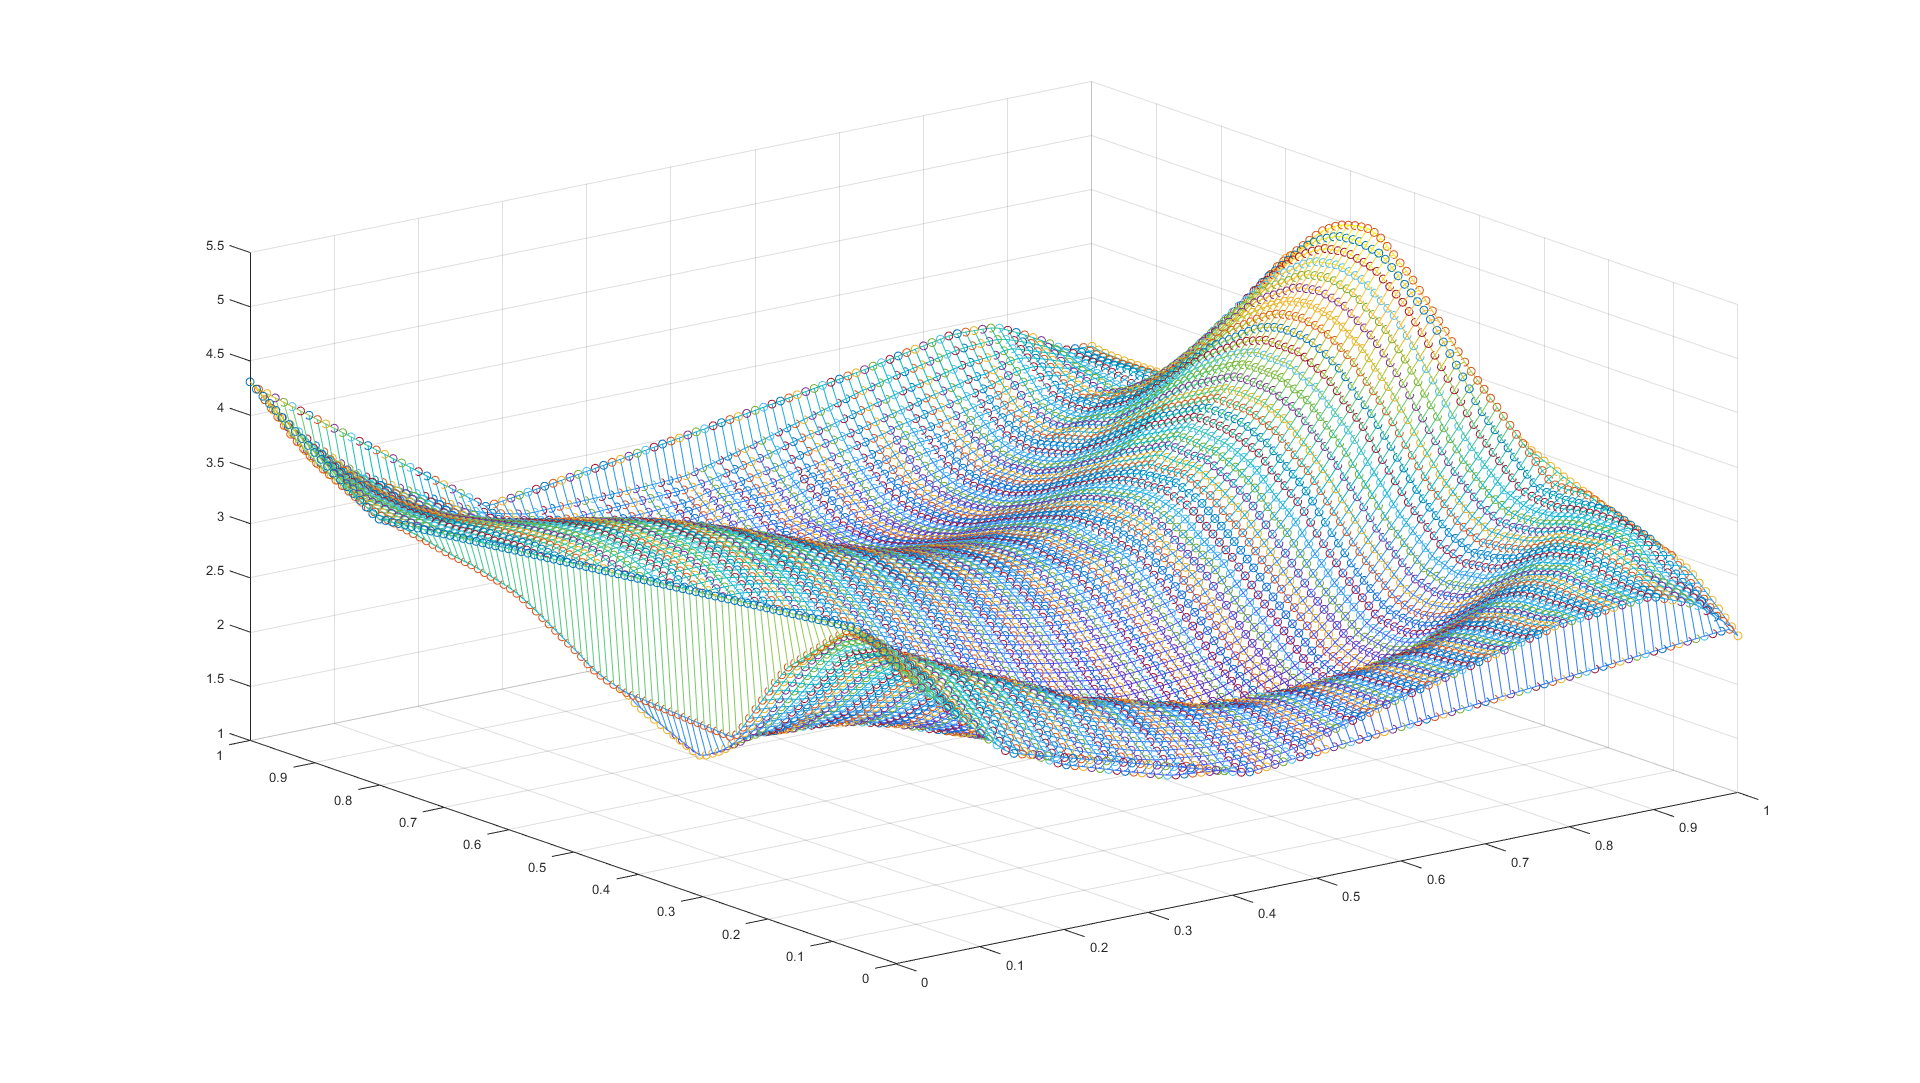
\includegraphics[width=0.4\textwidth]{surface.png}
	\caption{The visualization of the target surface of the training set.}
	\label{fig:surface}
\end{figure}


\textbf{Build and train your feedforward Neural Network: use the training and validation sets. Build the ANN with 2
	inputs and 1 output. Select a suitable model for the problem (number of hidden layers, number of neurons in
	each hidden layer). Select the learning algorithm and the transfer function that may work best for this problem.
	Motivate your decisions. When you try different networks, clearly say at the end which one you would select as
	the best for this problem and why.}\\

The feedforward neural network is build by using the Deep Learning Toolbox in Matlab. Table \ref{tab:design} shows an overview of design decisions that have been tried. Each combination is run $ 10 $ times from which the average mean square error is calculated. In order to deal with overfitting the validation set is used to perform early stopping. This means that during training the error on the validation set may only $ 10 $ increase directly after each other. If this amount is exceeded the learning is stopped. Early stopping is the default measure to deal with overfitting in the Matlab Deep Learning toolbox. Additionally, to avoid overfitting a regulation term is added in the objective function during training. This regulation term is the L2 norm of the weights and a regulation parameter is used to determine the importance of the regulation term in comparison with the training error on the targets.\\ The training is stopped when the max amount of $ 500 $ iterations is reached, the training error becomes smaller then $ 10^{-3} $ or when the learning takes longer then $ 1 $ minute. The activation functions that are used are the default ones of the Matlab toolbox. For a hidden layer and the output layer are respectively the ``tansig'' and ``purelin'' functions used.\\
It was found after simulations that the smallest average MSE on the validation set was found when the neural network has a regulation parameter of zero, two hidden layers of each five neurons and uses the gradient descent learning rule. \\


\begin{table}
	\centering
	\begin{tabular}{@{}lr@{}} \toprule
		\textbf{Design Variable}    & Domain \\\midrule
		Regulation parameter & $ 0 $ or $ 0.2 $  \\ 
		Amount of hidden layers & $ 1 $ or $ 2 $  \\
		Amount of neurons per layer & $ 5:5:100 $  \\
		Learning rule & all from Table \ref{tab:corr_no_noise}\\
		Training time per training session & $ 120 s $\\
		Max amount of epochs & $ 1000 $\\
		Max amount of sequential increases of the validation error & $ 10 $\\
		Goal of training error & $ 10^{-3} $\\
		Amount of iterations of average MSE & $ 10 $\\\bottomrule
	\end{tabular}
	\caption{The different design variable and their corresponding domain that were varied.}
	\label{tab:design}
\end{table}


\textbf{Performance Assessment: evaluate the performance of your selected network on the test set. Plot the surface of
	the test set and the approximation given by the network. Plot the error level curves. Compute the Mean Squared
	Error on the test set. Comment on the results and compare with the training performance. What else could you
	do to improve the performance of your network?}\\

Now the performance of the learned Neural Network is assessed on the test set. The chosen neural network is trained for $ 5 $ minutes.
Figure \ref{fig:After_simulation_of_5min_per} shows the distribution of the errors between target and prediction sets. A correlation coefficient of $ R = 98.3 $ is reached between target and prediction values which means there is almost a perfect correlation. It can be seen that at the end the error on the test set is smaller than the error on the training set. This is possible however, this is normally not the case because the test set is data that is never seen by the network before. The MSE error on respectively the training and the test set is $ 1.29 \times 10^{-2} $ and $ 1.12 \times 10^{-2} $. \\ 
Figure \ref{fig:errorSurface} shows the difference between the two planes by subtracting the learned plane from the target plane. It can be seen that especially in the middle the neural network did a better regression job than on the sides. 


% and Figure \ref{After_similation_of_5min} shows the correlation between the target and prediction values of the test set. It can be seen that there is a correlation coefficient of $ R = 98.3 $ which means there is almost a perfect correlation.\\ 


%Figure \ref{fig:After_simulation_of_5min} gives the evolution of the error on the training, validation and test set in function of the number of epochs during training.
%Figure \ref{fig:learnedSet} shows in red the target surface and in blue the learned surface. Figure \ref{fig:errorSurface} shows the difference between the two planes by subtracting the learned plane from the target plane. It can be seen that especially in the middle the neural network learned better predictions than on the sides. 

Things that could be done to improve the network are a more extensive parameter search and looking at the possibility to combine different learned networks. 


%\begin{figure}[h!]
%	\centering
%	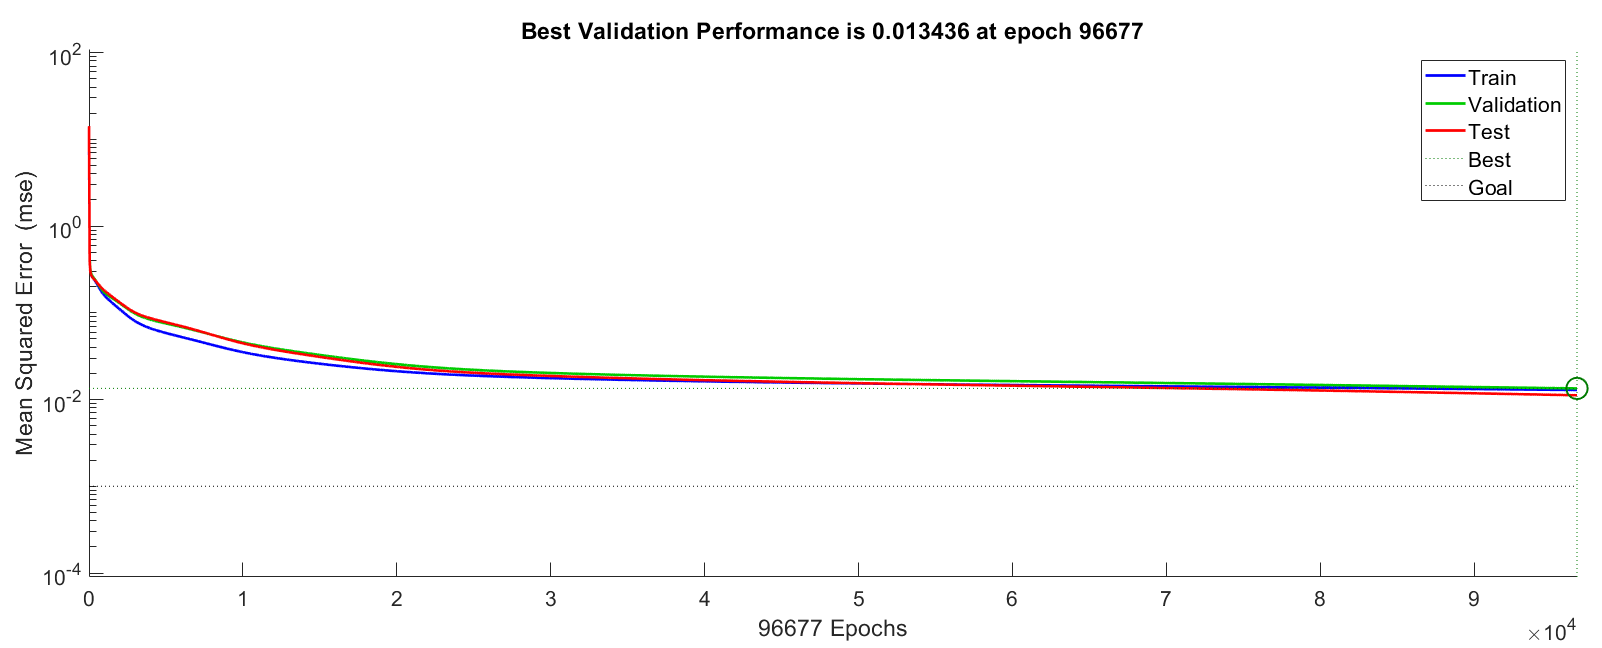
\includegraphics[width=1\textwidth]{After_simulation_of_5min.png}
%	\caption{The decrease of training, validation and test set error in function of the number of epochs.}
%	\label{fig:After_simulation_of_5min}
%\end{figure}

\begin{figure}[h!]
	\centering
	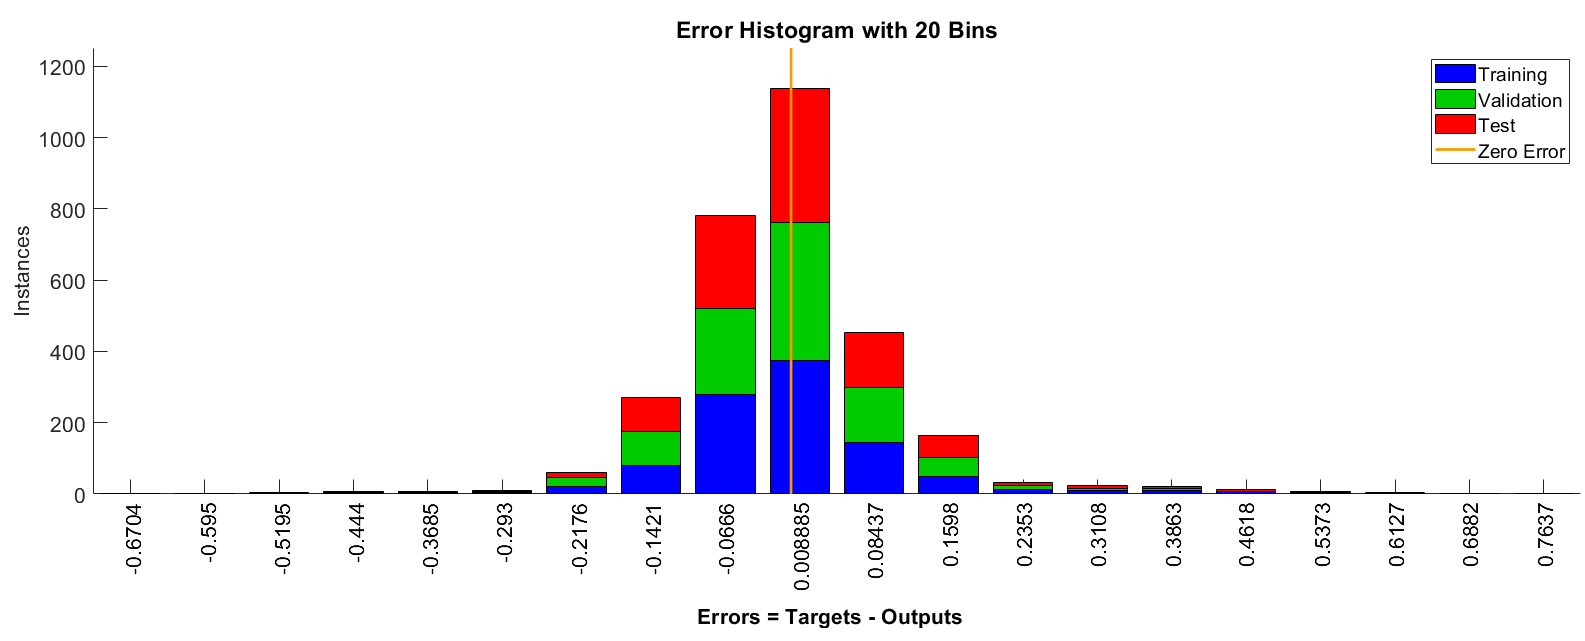
\includegraphics[width=1\textwidth]{After_simulation_of_5min_per.png}
	\caption{The distribution of the errors of the training, validation and test sets.}
	\label{fig:After_simulation_of_5min_per}
\end{figure}

%\begin{figure}[h!]
%	\centering
%	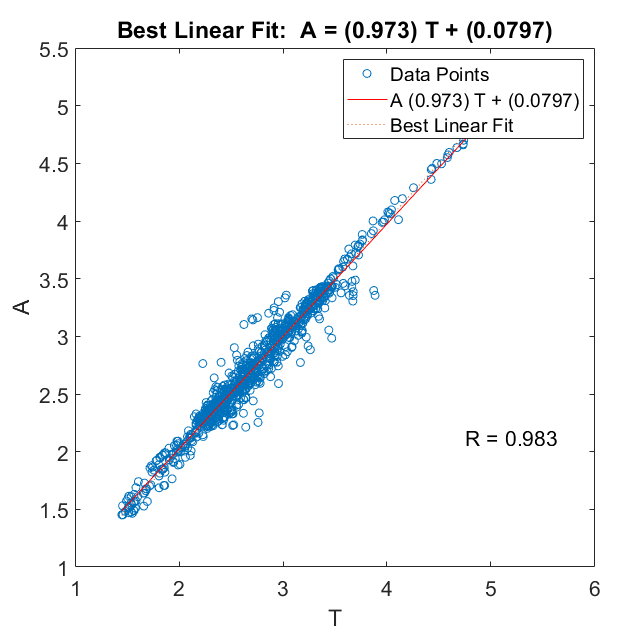
\includegraphics[width=0.5\textwidth]{After_similation_of_5min.png}
%	\caption{The correlation between the target and predicted values of the test set.}
%	\label{fig:After_similation_of_5min}
%\end{figure}


%\begin{figure}[h!]
%	\centering
%	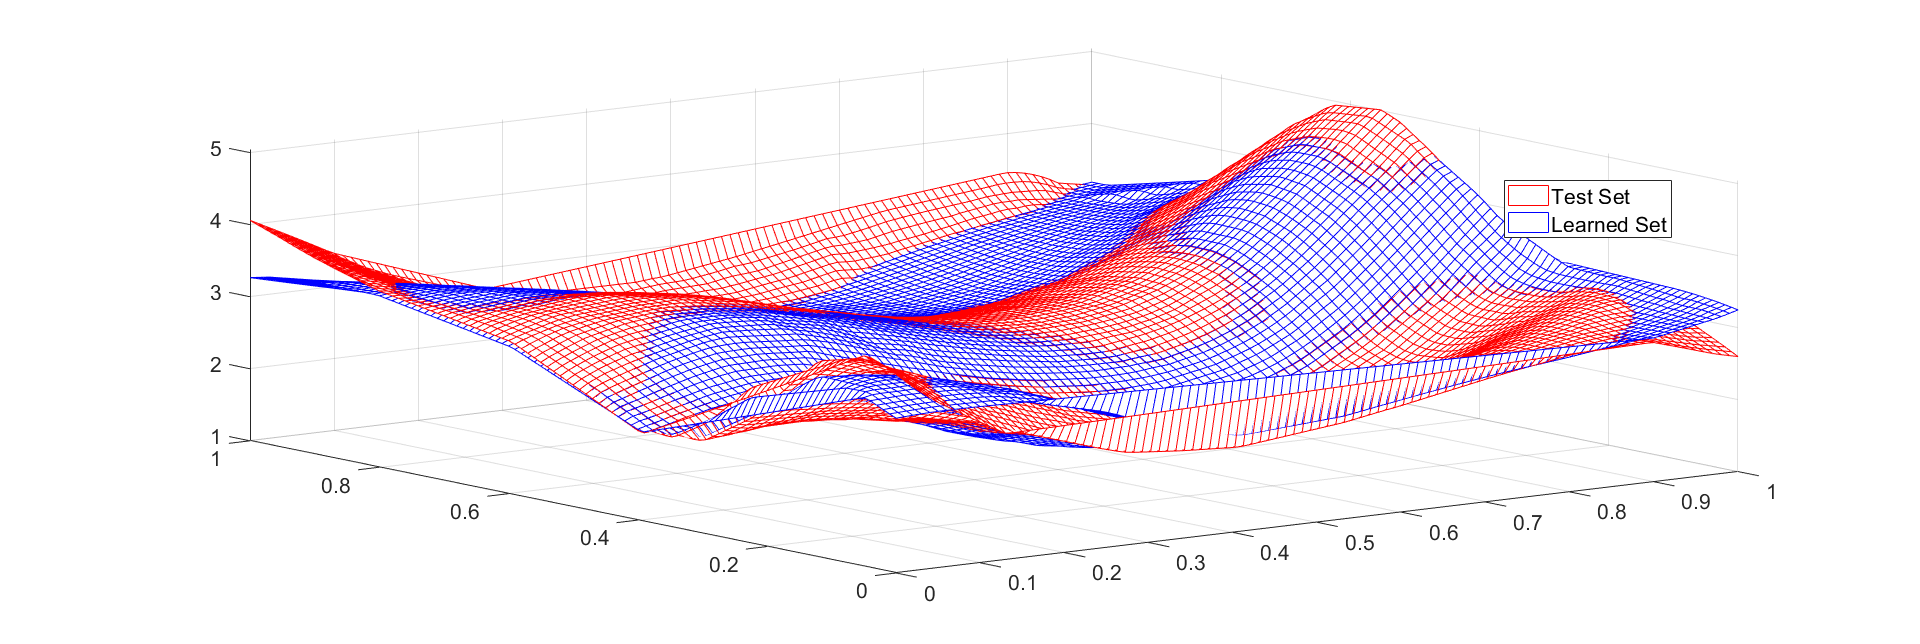
\includegraphics[width=0.8\textwidth]{learnedSet.png}
%	\caption{In red the target plane and in blue the learned plane are shown.}
%	\label{fig:learnedSet}
%\end{figure}

\begin{figure}[h!]
	\centering
	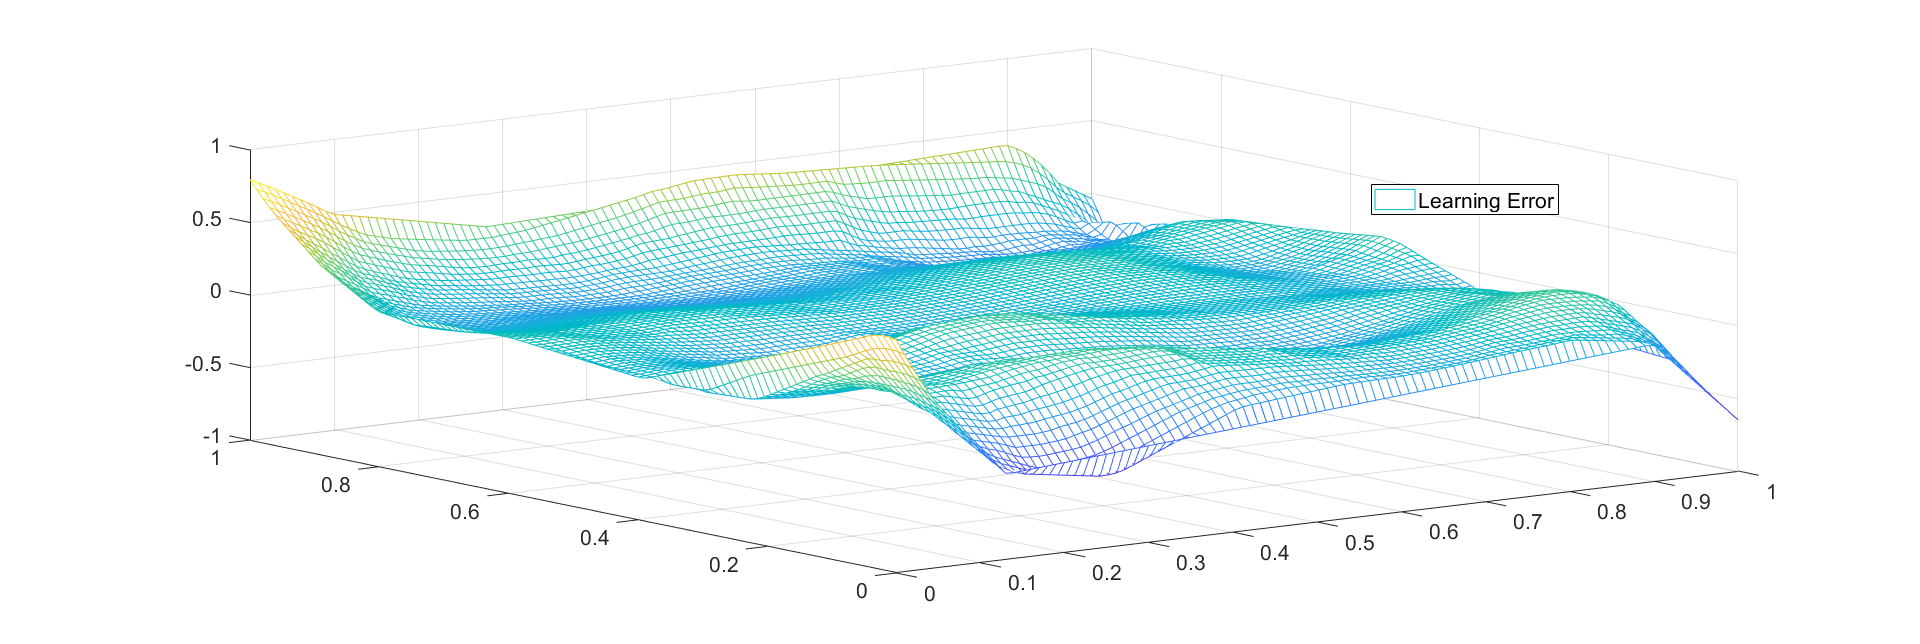
\includegraphics[width=0.6\textwidth]{errorSurface.png}
	\caption{The error plane that shows the difference between the target and the learned plane.}
	\label{fig:errorSurface}
\end{figure}


%\begin{figure}[h!]
%	\centering
%	\includegraphics[width=1.0\textwidth]{RNN.png}
%	\caption{Figure of the logical flow of a vanilla RNN with a hidden state (source \cite{Czum2020}).}
%	\label{fig:RNN}
%\end{figure}

%\begin{table}
%  \centering
%  \begin{tabular}{@{}llr@{}} \toprule
%    \multicolumn{2}{c}{Item} \\ \cmidrule(r){1-2}
%    Animal    & Description & Price (\$)\\ \midrule
%    Gnat      & per gram    & 13.65 \\
%              & each        & 0.01 \\
%    Gnu       & stuffed     & 92.50 \\
%    Emu       & stuffed     & 33.33 \\
%    Armadillo & frozen      & 8.99 \\ \bottomrule
%  \end{tabular}
%  \caption{A table with the correct layout.}
%  \label{tab:ok}
%\end{table}
\newpage
\section{Exercises of Section 5}
\textbf{Use trainbr to analyse the first two datasets of section 2 (the function y = sin(x2) and the noisy version) and compare it with the other training algorithms investigated there. Compare the test errors. Consider overparametrized networks (many neurons): do you see any improvement with trainbr?}\\

The Bayesian regularization backpropagation method already attains a good correlation coefficient after one epoch as can be seen in Tables \ref{tab:corr_no_noise} and \ref{tab:corr_with_noise}. This is similar as the ``Levenberg-Marquardt'' learning rule. However, the method distinguishes itself by taking a combination of the squared errors and weights into account from which the hyper parameters that determine the importance of both terms, are automatically obtained. Because now a regularization term is used it is expected that the Bayesian regularization backpropagation method can better deal with noisy data.This can also be seen in Table \ref{tab:corr_with_noise} where the bayesian regularization backpropagation method performs the best on noisy training data where it first had similar performance on training data without noise. \\ Tabel \ref{tab:over_para} gives the performance on an overparameterized network consisting of $ 1 $ hidden layer with $ 100 $ neurons and learning from noisy training data.  The effect of over parametrization between Table \ref{tab:over_para} and Table \ref{tab:corr_with_noise} can be seen on all methods except for the gradient descent methods. The calculation of the MSE is made by considering $ 3142 $ samples of the sinus function without noise.\\


\begin{table}
	\centering
	\begin{tabular}{@{}lr@{}} \toprule
		\textbf{Learning rule}  &  MSE \\\midrule
		\textbf{Gradient Descent}  &  $ 2.33\times10^{-1} $ \\
		\textbf{GD with adaptive learning rate}  & $ 2.11\times10^{-1} $  \\
		\textbf{Fletcher-Reeves}  & $ 3.10\times10^{-2} $ \\
		\textbf{Polak-Ribier}  & $ 3.3\times10^{-2} $  \\
		\textbf{BFGS}  &  $ 5.4\times10^{-2} $\\
		\textbf{Levenberg-Marquardt}  &  $ 5.40\times10^{-2} $\\ 
		\textbf{Bayesian Regularization Backpropagation}  & $ 3.80\times10^{-2} $ \\ \bottomrule
	\end{tabular}
	\caption{The resulting MSE making use of a neural network with a hidden layer of $ 100 $ neurons.}
	\label{tab:over_para}
\end{table}

%\cite{fast_alg}
%\cite{inver_over}

\bibliographystyle{abbrv}
%\bibliography{ANN1}

\end{document}
